\documentclass[17pt, t, lualatex]{beamer}



\title{Hidrodinámica de ríos}
\date{\today}
\institute[UJTL]{Universidad Jorge Tadeo Lozano}
\author{Ludwig Alvarado Becerra}

\usepackage{amsmath, amssymb, mathtools}
\usepackage[spanish]{babel}
\usepackage{biblatex}
\usepackage{hyperref}
\usepackage{xurl}

\addbibresource{referencias.bib}  % Make sure your .bib file is correctly named


\addbibresource{referencias.bib}

% Probably load as late as possible
% Other options are
% - engine=pdflatex to compile in pdfLaTeX (with different fonts),
% - mathshape=rm to use serif font for math,
% - mathsahpe=custom to not set any math font (so that you can define your own math fonts)
\usetheme[engine=lualatex, mathshape=sf, fontdir=kthpq-files/fonts/Figtree/]{kthpq}
\setmonofont{Bitstream Vera Sans Mono}[Scale=.9]

% Custom colors (see beamercolorthemecustom.sty for more details)
% \usecolortheme{custom}

% Modify the headline template: KTH-full, KTH-section-only, or KTH-frametitle-only.
% \setbeamertemplate{headline}[KTH-full]

% Custom footline
% \setfootline{left}{center}{right}

\begin{document}

\inserttitlepage

\section{Introducción}

\insertsectionpage

\begin{frame}{Introducción}
  \begin{block}{¿Qué es?}
  \end{block}

  \begin{columns}
    \begin{column}{.5\textwidth}
      \begin{itemize}
        \item La hidrodinámica estudia la dinámica de los fluidos a través de métodos matemáticos en forma diferencial de ecuaciones de continuidad y aceleración de fluidos.\cite{julien2018river}
        \item Tiene aplicaciones en ingeniería civil y ambiental para minimizar el impacto del hombre en un ecosistema. 
      \end{itemize}

      
    \end{column}

    \begin{column}{.5\textwidth}
      \begin{figure}[ht]
        \centering
        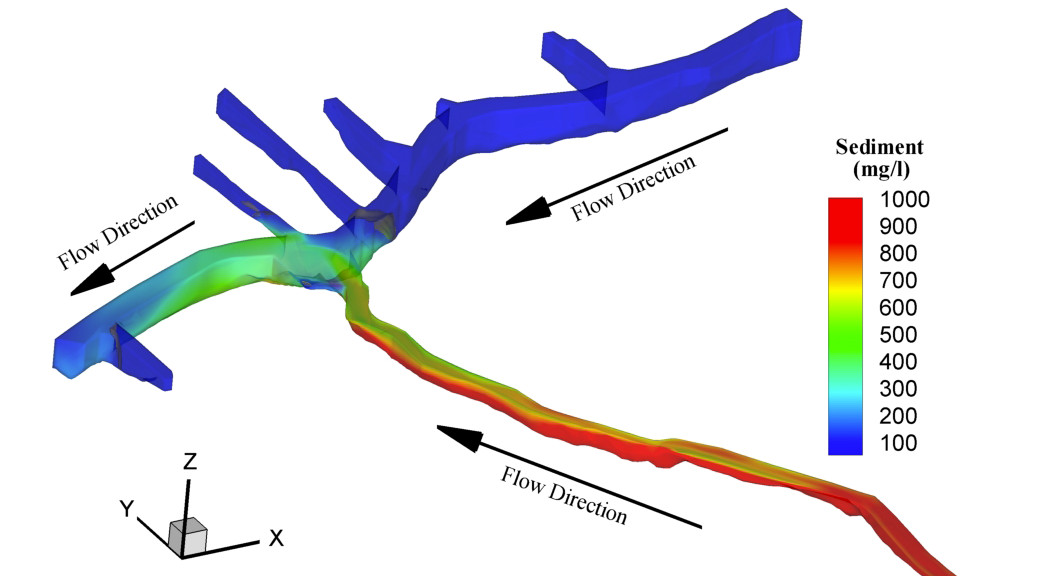
\includegraphics[width=0.8\textwidth]{img/1.jpg}
        \caption{\label{fig:1} Simulación de Ven Te Chow Hydrosystems Lab \parencite{ventechow2016river}.}
      \end{figure}

    \end{column}
  \end{columns}

\end{frame}

\section{Inspiración y motivación}

\insertsectionpage

\begin{frame}{Inspiración y motivación}

  \begin{columns}
    \begin{column}{.5\textwidth}
      \begin{itemize}
        \item Sistemas 1D y 2D.
        \item Fomentar interdisciplinariedad en el proyecto.
        \item Manejo de datos geoespaciales.
        \item Mi novia.
      \end{itemize}

      
    \end{column}

    \begin{column}{.5\textwidth}
      \begin{figure}[ht]
        \centering
        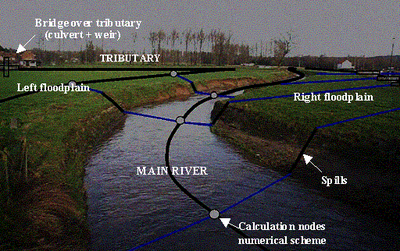
\includegraphics[width=0.8\textwidth]{img/2.png}
        \caption{\label{fig:2} Ejemplo de modelamiento \parencite{kuleuven_river_image}.}
      \end{figure}

    \end{column}
  \end{columns}

\end{frame}


\section{Objetivos}

\insertsectionpage

\begin{frame}{Objetivos}

  \begin{columns}
    \begin{column}{.4\textwidth}
      \begin{itemize}
        \item Apicar los conceptos de la clase de Sistemas Dinámicos en un proyecto con enfoque en datos geoespaciales.
        \item Un aplicativo interactivo que permita realizar simulaciones sobre la dinámica de un río específico.
        \item Expandir el conocimiento de problemáticas y situaciones medioambientales del autor. 
      \end{itemize}

      
    \end{column}

    \begin{column}{.6\textwidth}
      \begin{figure}[ht]
        \centering
        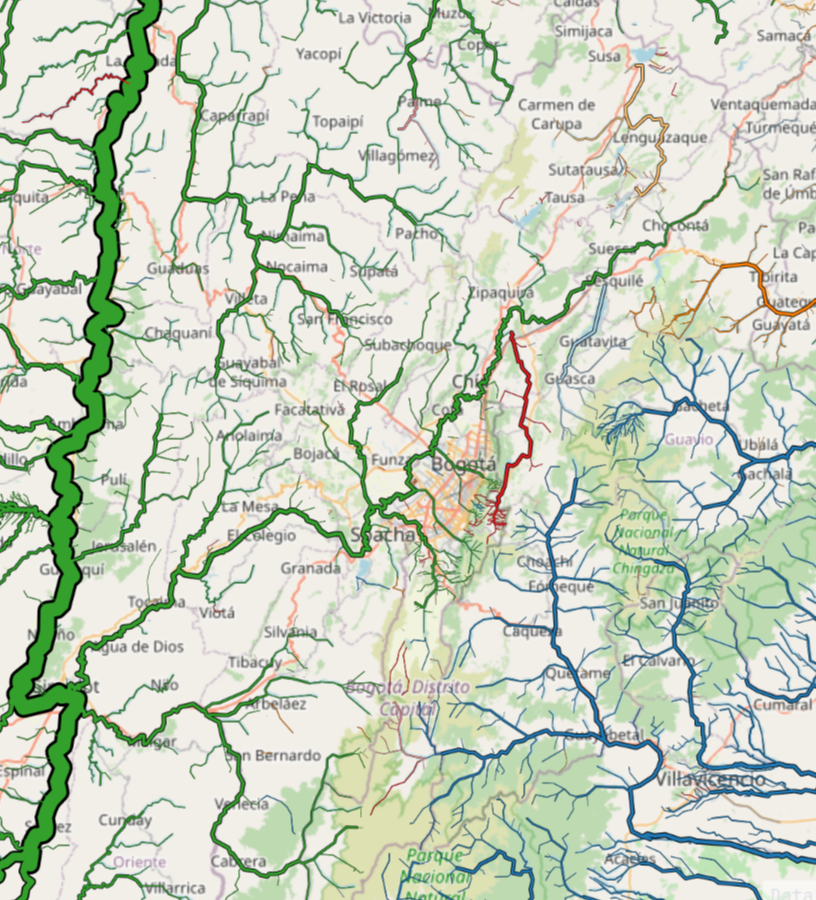
\includegraphics[width=0.45\textwidth]{img/3.png}
        \caption{\label{fig:3} Algunas Rutas hídricas de Colombia. Datos de OpenStreetMap\cite{waterwaymap}.}
      \end{figure}

    \end{column}
  \end{columns}

\end{frame}

\section{Revisión bibliográfica}

\insertsectionpage

\begin{frame}{Revisión bibliográfica}

  \begin{block}{\textit{Using dynamics for environmental modelling: Lessons learnt from six case studies}\cite{el2012using}}
  \end{block}

\begin{columns}
  \begin{column}{.5\textwidth}
    \begin{itemize}
      \item Revisión de algunos casos de aplicación de sistemas dinámicos en problemáticas ambientales.
      \item Aplicación de un juego interactivo. 
\end{itemize}
  \end{column}

  \begin{column}{.5\textwidth}
    \begin{figure}[ht]
      \centering
      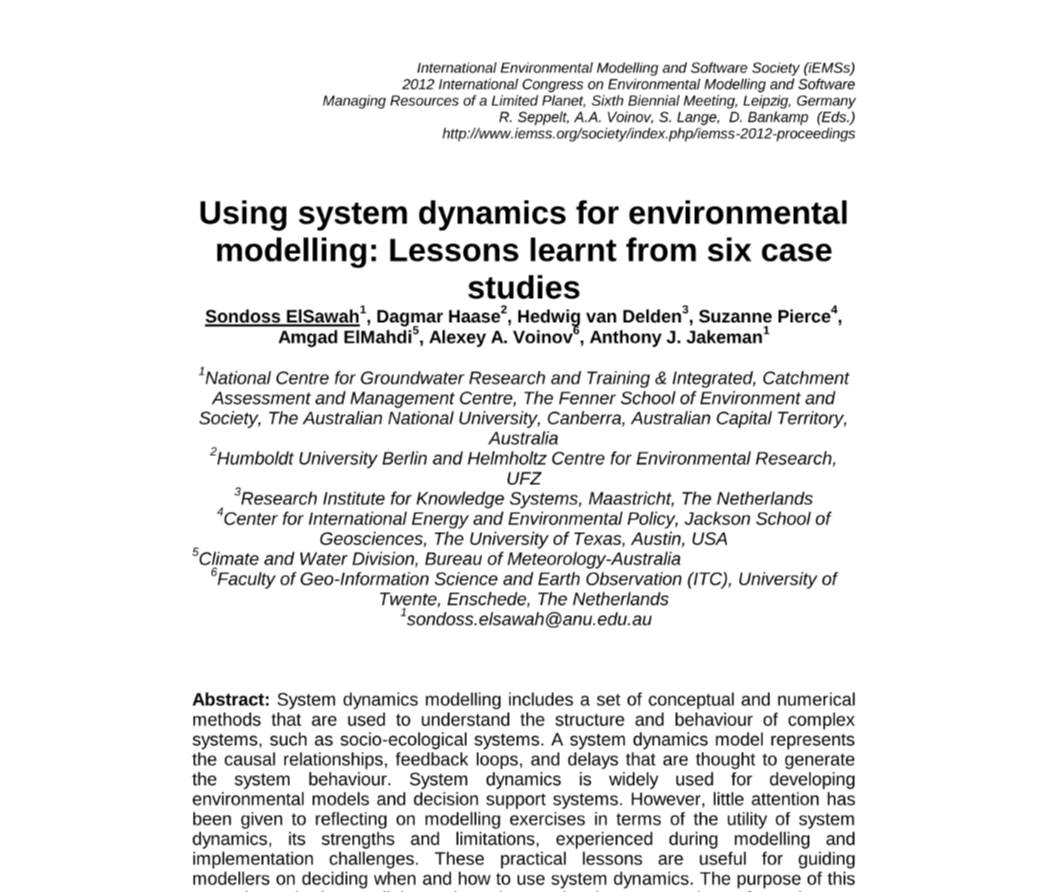
\includegraphics[width=0.65\textwidth]{img/4.png}
    \end{figure}
  \end{column}
\end{columns}

\end{frame}

\begin{frame}{Revisión bibliográfica}

  \begin{block}{\textit{Dynamic modeling of environmental systems}\cite{deaton1999dynamic}}
  \end{block}

\begin{columns}
  \begin{column}{.5\textwidth}
    \begin{itemize}
      \item Modelado mediante Sistemas Dinámicos con diferentes aplicaciones ambientales.
      \item Capítulo dedicado a hidrodinámica de ríos.
      \item Ejemplo de aplicación para el río Altamaha.
\end{itemize}
  \end{column}

  \begin{column}{.5\textwidth}
    \begin{figure}[ht]
      \centering
      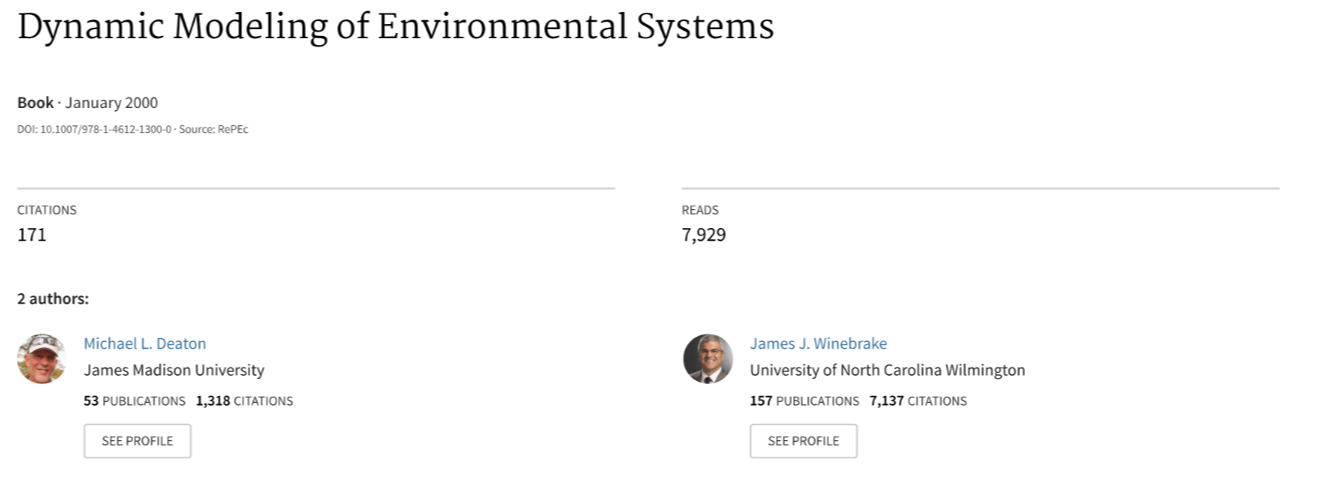
\includegraphics[width=1\textwidth]{img/5.png}
    \end{figure}
  \end{column}
\end{columns}

\end{frame}

\begin{frame}{Otros recursos encontrados}

\begin{itemize}
  \item \textit{Introduction to depth averaged modeling and user's manual}\cite{steffler2002introduction}.
  \item \textit{An Introduction to Hydrodynamics and Water Waves}\cite{le2013introduction}.
  \item \textit{Theory and Practice of Hydrodynamic Reconstruction in Plain River
Networks}
  \item \textit{Computational river dynamics}\cite{wu2007computational}.
  \item \textit{River mechanics}\cite{julien2018river}.
\end{itemize}

\end{frame}

\section{\textit{Datasets}}

\insertsectionpage

\begin{frame}[allowframebreaks]{\textit{Datasets}}

\begin{itemize}
  \item Modelo Digital de Elevación. Colombia \url{http://www.colombiaenmapas.gov.co/?e=-75.21433704101813,4.250807726576179,-65.21677844727078,10.458355638020791,4686&b=igac&l=159&u=0&t=23&servicio=159}
  \item Datos de ríos en Colombia \url{htts://www.openstreetmap.org}
  \item Obtener coeficientes de rugosidad de Mannings a través de publicaciones científicas.
\end{itemize}


\end{frame}




\section{Referencias}

\insertsectionpage
\begin{frame}[allowframebreaks]{Referencias}
  \printbibliography
\end{frame}


\insertendpage

\end{document}
